% Informe del Laboratorio 2 · NovaRetail 360.  Compilar desde la carpeta del laboratorio:  make informe
\documentclass[11pt,letterpaper]{article}
\usepackage{ud-informe}
\usepackage{amsmath}
\usepackage{array}
\usepackage[section]{placeins}   % las figuras no pasan de su sección
\newcolumntype{L}[1]{>{\raggedright\arraybackslash}p{#1}}
\setlength{\headheight}{22pt}
\graphicspath{{../capturas/}}

\renewcommand{\UDtitulo}{NovaRetail 360}
\renewcommand{\UDsubtitulo}{Modelamiento dimensional e indicadores: ¿se están cumpliendo las metas comerciales?}
\renewcommand{\UDtipo}{Laboratorio 2}
\renewcommand{\UDasignatura}{Inteligencia de Negocios}
\renewcommand{\UDdocente}{Nancy Yaneth Gelvez Garcia}
\renewcommand{\UDestudiantes}{Juan Felipe Rodríguez Galindo -- 20261595004 \\ & Carlos Stiven Mora Hoyos -- 20261595003}
\renewcommand{\UDencabezado}{Laboratorio 2 -- NovaRetail 360}

\newcommand{\cop}[1]{\$\,#1}
% Acento azul en lugar del rojo de la plantilla, como en el laboratorio 1 (combina con el logo MCIC).
\definecolor{udrojo}{HTML}{1291C0}
\definecolor{udrojoosc}{HTML}{085C83}
\hypersetup{linkcolor=udrojoosc, citecolor=udrojoosc, urlcolor=udrojoosc}
\newcommand{\destacar}[1]{{\color{udrojoosc}\bfseries #1}}
\newcommand{\VentasNetasTotal}{669.412.345}
\newcommand{\MetaTotal}{1.715.000.000}
\newcommand{\CumplTotal}{39{,}0\,\%}
\newcommand{\CeldasConciliadas}{30}
\newcommand{\DifMaxCelda}{0{,}00}
\newcommand{\DirectaCard}{* a *}
\newcommand{\DirectaFilas}{7.158}
\newcommand{\DirectaMeta}{409.825.000.000}
\newcommand{\DirectaNetas}{4.016.474.070}
\newcommand{\DirectaVecesMeta}{239{,}0}
\newcommand{\DirectaVecesNetas}{6{,}0}
\newcommand{\CumplRegMin}{37{,}2\,\%}
\newcommand{\CumplRegMax}{40{,}6\,\%}
\newcommand{\CumplMesMin}{35{,}4\,\%}
\newcommand{\CumplMesMax}{42{,}3\,\%}
\newcommand{\CumplCeldaMin}{24{,}4\,\%}
\newcommand{\CumplCeldaMax}{56{,}3\,\%}
   % cifras de la parte 4, escritas por modelo/modelo_estrella.py
\makeatletter\newcommand{\tablagenerada}[1]{\@@input #1 }\makeatother   % \input no sirve dentro de tabular

\begin{document}
\UDportada
\tableofcontents
\newpage

%=============================================================================
\section{Respuesta a la pregunta orientadora}

\textbf{No se están cumpliendo.} Las ventas netas del semestre suman \cop{\VentasNetasTotal} frente a una meta de
\cop{\MetaTotal}: un cumplimiento de \destacar{\CumplTotal}, y ninguna de las 30 combinaciones mes--región llega a la
meta. Lo que falta validar es la causa: todas las regiones quedan entre \CumplRegMin{} y \CumplRegMax, lo que apunta
más a cómo se fijó la meta que al desempeño de una región.

\medskip
Se trabajó sobre una copia diaria de la base del laboratorio 1, con DBeaver como cliente SQL. Como Power BI no
corre en macOS, la parte~4 se hizo en Python sobre los mismos ocho CSV.

%=============================================================================
\section{Parte 1. Reto con el modelo operacional}

\begin{enumerate}
  \item \textbf{Tablas y pasos:} cuatro tablas (ventas, clientes, devoluciones y metas) y tres pasos encadenados
        para una sola pregunta.
  \item \textbf{Por canal o por semana:} habría que reescribir casi toda la consulta, y aun así no hay metas por
        canal ni por semana para comparar.
  \item \textbf{Región:} la de una venta viene de \texttt{clientes} (la región actual del cliente, no la del momento
        de la compra); la de una meta está en \texttt{metas}, como texto.
\end{enumerate}

%=============================================================================
\section{Parte 2. Modelo estrella}

El script \texttt{clase1\_estrella\_PLANTILLA.sql} corre completo sin errores y tiene los cinco TODO
resueltos y los resultados de los controles al final.

\begin{table}[!ht]
\centering\small
\caption{Controles de nuestra base frente a la referencia.}
\begin{tabular}{llrr}
\toprule
Control & Medida & Nuestra base & Referencia \\
\midrule
C1 & Filas de FactVentas & 1\,193 & 1\,192 \\
C2 & Ventas netas & 669\,412\,345 & 668\,833\,145 \\
C2 & Meta total & 1\,715\,000\,000 & 1\,715\,000\,000 \\
C4 & Meta inflada & 68\,322\,000\,000 & 68\,262\,000\,000 \\
C5 & Cumplimiento / devolución / descuento & 39,03 / 4,15 / 5,09\,\% & 39,0 / 4,15 / 5,10\,\% \\
\bottomrule
\end{tabular}
\end{table}

\textbf{Diferencia con la referencia.} Es una sola venta, V00410 (\cop{579\,200}): venía con precio negativo y en el
laboratorio 1 la corregimos con el precio de lista; la referencia la rechaza. Las demás tablas coinciden.

\paragraph{¿Por qué FactMetas no se une con FactVentas?} Tienen granos distintos (mes por región frente a línea de
venta). Al unirlas, la meta se repite en cada venta: C4 da 68\,322 millones, casi 40 veces la meta real.

\paragraph{¿Por qué DimFecha y DimPeriodo son dos tablas?} Las metas solo existen por mes. DimPeriodo es la
dimensión compartida a ese grano y DimFecha (día) se conecta a ella.

\paragraph{¿Para qué sirve \texttt{sk\_cliente}?} Permite guardar varias versiones de un mismo cliente (tipo 2) y
que cada venta apunte a la versión vigente en su fecha.

%=============================================================================
\section{Parte 3. Cambios en dimensiones}

Caso: C0005 pasa de Bogotá a Medellín el 1 de abril. Compró en enero, febrero y mayo.

\begin{enumerate}
  \item \textbf{Tipo 1:} sus compras de enero a marzo quedan en Medellín. No sirve para las metas de Bogotá, que
        pierde ventas reales (en febrero baja de 36,1\,\% a 33,5\,\%).
  \item \textbf{Tipo 2:} se crea una nueva versión del cliente (sk 121) y la anterior se cierra el 31 de marzo.
        Las fechas de vigencia indican qué versión aplica a cada venta, así la historia se conserva.
  \item \textbf{Ejemplo de tipo 1:} corregir un error de digitación en un nombre.
\end{enumerate}

%=============================================================================
\section{Parte 4. Modelo (Python en lugar de Power BI)}

Se importaron los ocho CSV, se crearon las ocho relaciones y se calcularon las tres medidas (Ventas Netas, Meta y
\% Cumplimiento). Todas las relaciones son de uno a varios, con filtro de la dimensión al hecho.

\begin{figure}[!ht]
\centering
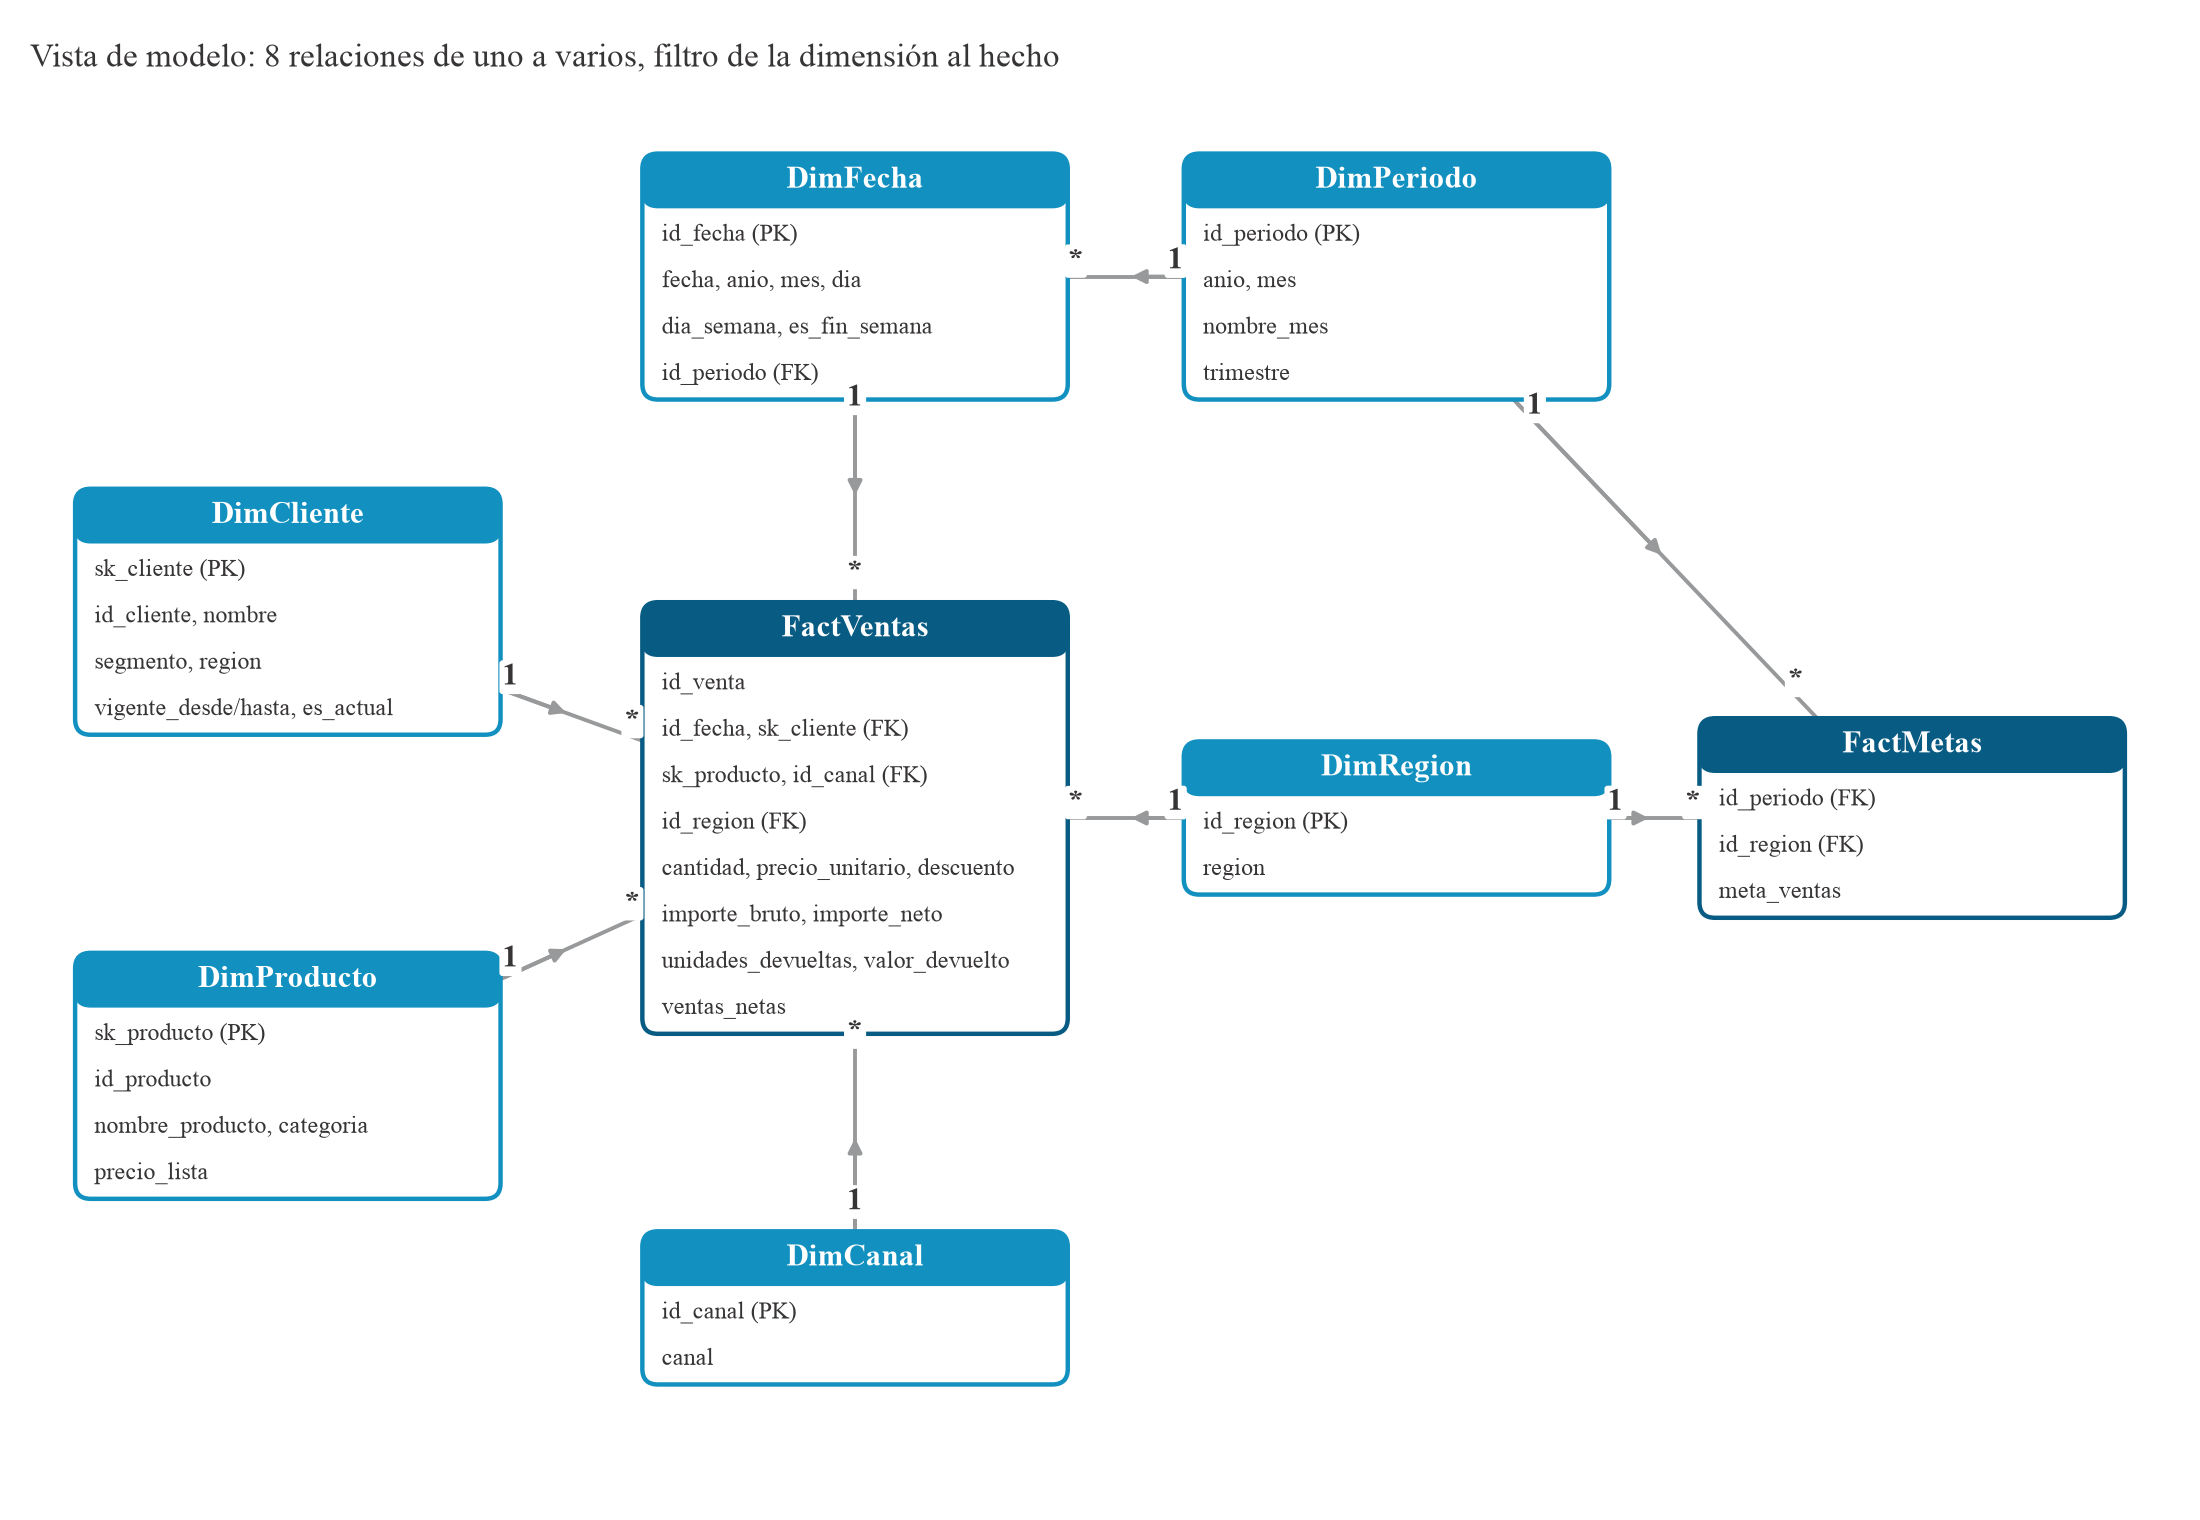
\includegraphics[width=0.92\textwidth]{vista_modelo.png}
\caption{Vista del modelo.}
\end{figure}

\begin{table}[!ht]
\centering\small
\caption{\% Cumplimiento por región y mes.}
\label{tab:matriz}
\begin{tabular}{lrrrrrrr}
\toprule
Región & Enero & Febrero & Marzo & Abril & Mayo & Junio & Total \\
\midrule
\tablagenerada{generado/matriz.tex}
\bottomrule
\end{tabular}
\end{table}

La matriz coincide celda por celda con el control C3 y el total con C2.

\textbf{Si se relaciona FactMetas con FactVentas} la relación queda de varios a varios y la meta se multiplica
(\DirectaVecesMeta{} veces la real), así que se borró.

%=============================================================================
\section{Parte 5. Catálogo de KPI}

\begin{table}[!ht]
\centering\small
\caption{Resumen del catálogo (detalle en el Excel).}
\begin{tabular}{L{4.2cm}rL{4.4cm}}
\toprule
Indicador & Valor & Meta \\
\midrule
K1 Cumplimiento de la meta & 39,0\,\% & 100\,\% (de la empresa) \\
K2 Tasa de devolución & 4,15\,\% & $\le$ 4\,\% (propuesta del equipo) \\
K3 Descuento efectivo & 5,09\,\% & $\le$ 5\,\% (propuesta del equipo) \\
K4 Ticket promedio neto & \cop{561\,117} & Sin meta \\
\bottomrule
\end{tabular}
\end{table}

\begin{enumerate}
  \item \textbf{¿Cuál no es todavía un KPI?} K4: no tiene meta, umbrales ni responsable.
  \item \textbf{¿K1 habla de las regiones o de la meta?} Más de la meta: regiones y meses quedan todos cerca del
        40\,\%. Es una hipótesis que hay que validar con la gerencia.
\end{enumerate}

%=============================================================================
\section{Conclusiones}

\begin{enumerate}
  \item Las metas no se cumplen: \CumplTotal{} en el semestre.
  \item La brecha es pareja en todas las regiones, así que hay que revisar cómo se fijó la meta.
  \item Las dos tablas de hechos solo se comparan a través de las dimensiones; unirlas directamente infla la meta.
  \item El tipo 2 conserva la historia del cliente; el tipo 1 la reescribe.
\end{enumerate}

\end{document}
